\section{Вариационный принцип Гамильтона}

Можно сказать, что есть пространство, проводить кривые, а потом их друг с другом сравнивать. Пусть есть некоторое конфигурационное многообразие $M$ с $\dim M = n$ и частицами $q_1,\ldots, q_n$. 

Пусть $\gamma(t)$ соединяет $q_0$ и $q_1$. 
Что мы точно знаем? Знаем, что $\gamma(t_0) = q^0$ и что $\gamma(t_1)=q^1$. Введем некоторый функционал
\begin{equation}
    S = \int_{t_0}^{t_1} L(\gamma(t), \dot{\gamma}(t), t) \d t
    \hspace{0.5cm} 
    \text{--- \textit{действие по Гамильтону}}.
\end{equation}
Переходя к однопараметрическому семейству кривых $\gamma(\alpha, t)$, где $\alpha$ -- скалярный параметр. Тогда
\begin{equation}
    S = \int_{t_0}^{t_1} L(\gamma(\alpha, t), \dot{\gamma}(\alpha, t), t) \d t
    \hspace{0.5cm} 
    \delta S = \frac{d S}{d \alpha} d \alpha 
    \hspace{0.5cm} 
    \text{--- \textit{вариация действия}}.
\end{equation}

\begin{to_thr}[принцип Гамильтона]
     Кривая $\gamma(\alpha, t)$ является экстремалью функционала тогда и только тогда, когда является решением уравнений Лагранжа. 
     \begin{equation}
         \delta S = 0
         \hspace{0.5cm} \Leftrightarrow \hspace{0.5cm} 
         \gamma(\alpha, t) \in \Sol(\text{ур-ний Лагранжа})
     \end{equation}
\end{to_thr}


\begin{proof}[$\triangle$]
    Давайте просто проварьируем Лагранжиан, тогда
    \begin{equation*}
        \delta S = \int_{t_0}^{t_1} 
        \left(
            \frac{\partial L}{\partial q_i} \frac{\partial q_i}{\partial \alpha} +
            \frac{\partial L}{\partial \dot{q}_i} \frac{\partial \dot{q}_i}{\partial \alpha}  
        \right) \delta \alpha \d t =
        \ldots
        =
        \int_{t_0}^{t_1}
        \left(
            \frac{d}{dt} \frac{\partial L}{\partial \dot{q}_k} - \frac{\partial L}{\partial q_k}
        \right) \delta q_k \d t = 0,  \hspace{0.5cm} k = 1, \ldots, n
    \end{equation*}
    таким образом уравнения Лагранжа выполнены. 
\end{proof}


\subsection{Опять маятник}



Посмотрим на маятник
\begin{equation*}
    L = \frac{1}{2} \left(\vphantom{\frac{1}{2}} \dot{q}^2 - q^2 \right),
\end{equation*}
где $q(0)=0, \ q(t_1)=q_1$. Получим различные ситуации. 

Подставив в уравнение Лагрнажа лагранжиан системы получим
\begin{equation*}
    \ddot{q} + q = 0
    \hspace{0.5cm} \Rightarrow \hspace{0.5cm} 
    q = A \cos t + B \sin t,
    \hspace{0.5cm} A = 0, \ q_1 = B \sin t_1.
\end{equation*}

\begin{wrapfigure}{r}{0.2\textwidth}
  \begin{center}
        \vspace{-5 mm}
        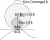
\includegraphics[width=0.8\linewidth]{figures/1.png}
  \end{center}
    %\caption{}
    %\label{fig:}
\end{wrapfigure}


\noindent
Пусть $t_1 \neq \pi k $ тогда $\exists ! B = q_1 / \sin t_1$. Но, если $t_1 = \pi k$ то при $q_1 \equiv 0 \ \forall B$ у нас решение (их $\infty$). Если же $q_1 \neq 0$ то не решение $\nexists$. 


\begin{to_def} 
    Есть на конфигурационном многообразие \textit{кинетические фокусы}. Если мы ставим краевую задачу до фокуса Якоби, то $\delta S = 0$ -- минимум, а иначе говорить не о чем, только экстремальность.   
\end{to_def}


%%%%%%%%%%%%%%%%%%%%%%%%%%%%%%%%%%%%%%%%%%%%%%%%%%%%%%%%%%%%%%%%%%%%%%%%%%%%%%%%%%%
\subsection{Бусинка на прямой}

Пусть $q(t)$ -- прямой путь, $q + \delta q$ -- окольный путь, вариация прямого пути. Рассмотрим такой интеграл
\begin{align*}
    S_{\text{ок}} - S_{\text{пр}} &= 
    \int_{t_0}^{t_1} \frac{1}{2} 
    \left(
        \dot{(q + \delta q)}^2 + (q + \delta q)^2 - \dot{q}^2 - q^2
    \right) \d t =
    \int_{t_0}^{t_1}
    \left(
        \dot{q} \delta \dot{q} + q \delta q + \frac{1}{2} \delta q^2  + \frac{1}{2} \delta \dot{q}^2 
    \right) \d t = \\
    &= \int_{t_0}^{t_1}  \frac{1}{2}  \left(
       \delta q^2 + \delta \dot{q}^2
    \right) +
    \int_{t_0}^{t_1} 
    \underbrace{\frac{1}{2} \delta (\dot{q}^2 + q^2)}_{0}
     \d t > 0
\end{align*}
ожидая всюду увидеть его положительным и, действительно, видя.

\subsection{Стационарная система}

Пусть есть некоторая система такая, что
\begin{equation*}
    \vc{v}_i =  \frac{\partial \vc{r}_i}{\partial q_k} \dot{q}_k,
    \hspace{0.5cm} \Pi \equiv 0.
\end{equation*}
Тогда Лагранжиан
\begin{equation}
    L = T_2 + \cancel{T_1} + \cancel{T_0} = \frac{1}{2} a_{ik} (q) \dot{q}^i \dot{q}^k.
\end{equation}
По принципу Гамильтона
\begin{equation*}
    \delta S = \delta \int \frac{1}{2} a_{ik} \dot{q}_i \dot{q}_k = 0,
\end{equation*}
хотим заменить $L \to \sqrt{2L}$, утверждается, что все стационарные точки сохранятся. Тогда
\begin{equation*}
    \delta S' = \delta \int \sqrt{2L} \d t = 
    \delta \int \sqrt{a_{ik}(q) \d q_i \d q_k} = \delta \int \d S.
\end{equation*}
то есть метрика образована кинетической энергией, получается решение уравнений Лагранжа это просто уравнение геодезической. Вот и кратчайший путь на многообразии. 

\subsection{Геодезические на сфере}

Начальные условия
\begin{equation*}
    \theta(0) = \frac{\pi}{2},  \ \varphi(0) = 0, \ \theta(0) = 0, \ \dot{\varphi}(0) = \dot{\varphi}_0
\end{equation*}
На сфере, в сферических координатах
\begin{equation*}
    L = \frac{1}{2} \left(
        \dot{\theta}^2 + \dot{\varphi}^2 \sin^2 \theta
    \right)
    \hspace{0.5cm} \Rightarrow \hspace{0.5cm} 
    S' = \int \sqrt{d \theta^2 + \sin^2 \theta \d \varphi^2}.
\end{equation*}
Также знаем, что
\begin{equation*}
    \frac{\partial L}{\partial \dot{\varphi}} = \const = \dot{\varphi} \sin^2 \theta,
    \hspace{0.5cm} 
    \ddot{\theta} + \dot{\varphi} \frac{1}{2} \sin 2 \theta  = 0.
\end{equation*}
Так получим
\begin{equation*}
    S' = \dot{\varphi}_0 (t_1 - t_0), 
\end{equation*}


\subsection{Равновесие. Принцип виртуальных перемещений.}


\begin{to_thr} [принцип Даламбера-Лагранжа]
Верно, что
\begin{equation*}
    m_i \vc{\mathrm{w}}_i = \vc{F}_i + \vc{R}_i,
    \hspace{0.5cm} \Rightarrow \hspace{0.5cm} 
    \sum_i \left(
        m_i \vc{\mathrm{w}}_i
    \right) \cdot \delta \vc{r}_i = 0.
\end{equation*}
\end{to_thr}


\begin{to_def} 
    Пусть $q^0 \in M$ -- точка равновесия, если при $\dot{q}^0 \equiv \dot{q}(0) \equiv 0$ приводит к $q(t) = q^0$. 
\end{to_def}

\begin{to_lem} 
    Для того, чтобы точка была положением равновесия необходимо и достаточно, чтобы сумма элементарных работ на $\forall$ виртуальных перемещениях всех активных сил была равна нулю.
    \begin{equation*}
        \delta A \bigg|_0 = 0
        \hspace{0.5cm} 
        \delta A = \sum_i \vc{F}_i \cdot \delta \vc{r}_i.
    \end{equation*}
\end{to_lem}

Этот принцип можно рассматривать, как дракона с тремя головами. Вот если система \textbf{голономная}, то
\begin{equation*}
    \delta A = Q_i \delta q_i 
    \hspace{0.5cm} \Rightarrow \hspace{0.5cm} 
    Q_i = 0 \ \forall i.
\end{equation*}
Если система \textbf{консервативная}, то
\begin{equation*}
    Q_1 = - \frac{\partial P}{\partial q^i} 
    \hspace{0.5cm} \Rightarrow \hspace{0.5cm} 
    \text{положение равновесия --- стационарная точка потенциала}.
\end{equation*}
Если же у нас \textbf{твёрдое тело}, тогда
\begin{equation*}
    \delta A = \left(
        \vc{R}^{\text{внеш}} \cdot \vc{v}_O
    \right) \d t + 
    \left(
        \vc{M}_O^{\text{внеш}} \cdot \vc{\omega}
    \right) dt
    \hspace{0.5cm} \Rightarrow \hspace{0.5cm} 
    \left\{\begin{aligned}
        \vc{R}^{\text{внеш}} &= 0 \\
        \vc{M}^{\text{внеш}} &= 0 \\
    \end{aligned}\right.
\end{equation*}


